\documentclass[11pt,a4paper]{article}
% ============================================================
% Shared preamble for Claude Experiments reports (Ukrainian, LuaLaTeX)
% Compile with: lualatex report_*_uk.tex
% Include this AFTER \documentclass in each report:
%   \documentclass[11pt,a4paper]{article}
%   % ============================================================
% Shared preamble for Claude Experiments reports (Ukrainian, LuaLaTeX)
% Compile with: lualatex report_*_uk.tex
% Include this AFTER \documentclass in each report:
%   \documentclass[11pt,a4paper]{article}
%   % ============================================================
% Shared preamble for Claude Experiments reports (Ukrainian, LuaLaTeX)
% Compile with: lualatex report_*_uk.tex
% Include this AFTER \documentclass in each report:
%   \documentclass[11pt,a4paper]{article}
%   \input{../preamble_uk}
% ============================================================
% Cyrillic via LuaLaTeX + fontspec (pdflatex has no T2A here).
\usepackage{fontspec}
\setmainfont{DejaVu Serif}
\setsansfont{DejaVu Sans}
\setmonofont{DejaVu Sans Mono}
\usepackage[a4paper,top=2.5cm,bottom=2.5cm,left=2.5cm,right=2.5cm]{geometry}
\usepackage{amsmath,amssymb}
\usepackage{graphicx}
\usepackage{subcaption}
\usepackage{booktabs}
\usepackage{xcolor}
\usepackage[colorlinks=true,allcolors=blue]{hyperref}
\usepackage{microtype}
\usepackage{float}
\usepackage{array}
\microtypesetup{expansion=false}

% Color scheme
\definecolor{colMicro}{HTML}{222222}
\definecolor{colExact}{HTML}{2878b5}
\definecolor{colPlacement}{HTML}{e07a1f}
\definecolor{colBoundary}{HTML}{429c74}
\definecolor{colCurrent}{HTML}{c23b55}
\definecolor{colMM}{HTML}{c23b55}

\providecommand{\SIG}{\textcolor{green!50!black}{\textbf{*}}}
\providecommand{\NS}{\textcolor{gray}{n.s.}}
\providecommand{\DRMS}{\Delta\mathrm{RMST}}
\providecommand{\ci}[2]{$[{#1},\;{#2}]$}

% ============================================================
% Cyrillic via LuaLaTeX + fontspec (pdflatex has no T2A here).
\usepackage{fontspec}
\setmainfont{DejaVu Serif}
\setsansfont{DejaVu Sans}
\setmonofont{DejaVu Sans Mono}
\usepackage[a4paper,top=2.5cm,bottom=2.5cm,left=2.5cm,right=2.5cm]{geometry}
\usepackage{amsmath,amssymb}
\usepackage{graphicx}
\usepackage{subcaption}
\usepackage{booktabs}
\usepackage{xcolor}
\usepackage[colorlinks=true,allcolors=blue]{hyperref}
\usepackage{microtype}
\usepackage{float}
\usepackage{array}
\microtypesetup{expansion=false}

% Color scheme
\definecolor{colMicro}{HTML}{222222}
\definecolor{colExact}{HTML}{2878b5}
\definecolor{colPlacement}{HTML}{e07a1f}
\definecolor{colBoundary}{HTML}{429c74}
\definecolor{colCurrent}{HTML}{c23b55}
\definecolor{colMM}{HTML}{c23b55}

\providecommand{\SIG}{\textcolor{green!50!black}{\textbf{*}}}
\providecommand{\NS}{\textcolor{gray}{n.s.}}
\providecommand{\DRMS}{\Delta\mathrm{RMST}}
\providecommand{\ci}[2]{$[{#1},\;{#2}]$}

% ============================================================
% Cyrillic via LuaLaTeX + fontspec (pdflatex has no T2A here).
\usepackage{fontspec}
\setmainfont{DejaVu Serif}
\setsansfont{DejaVu Sans}
\setmonofont{DejaVu Sans Mono}
\usepackage[a4paper,top=2.5cm,bottom=2.5cm,left=2.5cm,right=2.5cm]{geometry}
\usepackage{amsmath,amssymb}
\usepackage{graphicx}
\usepackage{subcaption}
\usepackage{booktabs}
\usepackage{xcolor}
\usepackage[colorlinks=true,allcolors=blue]{hyperref}
\usepackage{microtype}
\usepackage{float}
\usepackage{array}
\microtypesetup{expansion=false}

% Color scheme
\definecolor{colMicro}{HTML}{222222}
\definecolor{colExact}{HTML}{2878b5}
\definecolor{colPlacement}{HTML}{e07a1f}
\definecolor{colBoundary}{HTML}{429c74}
\definecolor{colCurrent}{HTML}{c23b55}
\definecolor{colMM}{HTML}{c23b55}

\providecommand{\SIG}{\textcolor{green!50!black}{\textbf{*}}}
\providecommand{\NS}{\textcolor{gray}{n.s.}}
\providecommand{\DRMS}{\Delta\mathrm{RMST}}
\providecommand{\ci}[2]{$[{#1},\;{#2}]$}


\title{\textbf{Synchronization audit: production MicroMacro проти event-driven scheduler}\\[0.4em]
\large Розмежування model abstraction та implementation discrepancy}
\author{Claude Experiments Series}
\date{7 серпня 2026}

\begin{document}
\sloppy
\maketitle

\begin{abstract}
У 100 парних реплікаціях при $T_{\mathrm{end}}=4000$ event-driven
aggregate/uniform scheduler мав $\Delta\mathrm{RMST}=-220.79$ відносно Full
Micro, тоді як production MicroMacro при
$\tau_{\mathrm{micro}}\in\{0.25,0.5,1\}$ мав зміщення від $-1228.03$ до
$-1259.18$. Відносно event-driven scheduler додаткове раннє зміщення
production variants становило $-1007.23$--$-1038.39$, і всі відповідні 95\%
CI виключали нуль. Відмінність між реалізаціями значно більша за зміну point
estimate між трьома перевіреними кроками. Оскільки production і event-driven
paths мають різні семантики, результат не є чистим quadrature study і не
підтримує твердження про границю $\tau\to0$. Completion усіх варіантів дорівнює 1.
\end{abstract}

\tableofcontents
\clearpage

\section{Статус і походження даних}\label{sec:status}

Повний аудит завершено для 100 парних реплікацій при єдиному горизонті
$T_{\mathrm{end}}=4000$. Full Micro і event-driven aggregate/uniform варіант
повторно використано з CE-01. Production MicroMacro запущено при
$\tau_{\mathrm{micro}}=0.25$, $0.5$ та $1$ на тих самих мережах і початкових
вузлах із детермінованими model-specific streams. Усі варіанти досягли
термінального шару в усіх прогонах. Збережено компактні arrival records,
але не повні траєкторії.

\section{Наукове питання}\label{sec:question}

Наскільки велика додаткова похибка production MicroMacro відносно event-driven
реалізації aggregate/uniform hazard model? Чи є дані в перевіреному діапазоні
$\tau_{\mathrm{micro}}$ достатніми, щоб приписати цю похибку лише кроку
синхронізації? Науковим пріоритетом є відокремити model abstraction error від
implementation/synchronization discrepancy, а не оцінювати runtime.

\section{Дизайн та оцінювана величина}\label{sec:design}

Порівняно:
\begin{itemize}
  \item \texttt{FullMicro} --- повну мережеву Gillespie CTMC;
  \item \texttt{EventDrivenAggregate} --- event-driven scheduler з
  aggregate hazard і uniform placement;
  \item \texttt{ProductionMM\_tau0.25}, \texttt{ProductionMM\_tau0.5} та
  \texttt{ProductionMM\_tau1} --- production midpoint/synchronization paths.
\end{itemize}

Full Micro є референсом для повної апроксимаційної похибки. Event-driven
aggregate scheduler є внутрішнім референсом для різниці між реалізаціями
aggregate model. Для кожного контрасту
\[
 \begin{aligned}
 \Delta\mathrm{RMST}
   &=\mathrm{RMST}_{\mathrm{variant}}-\mathrm{RMST}_{\mathrm{reference}},\\
 \Delta\mathrm{RMST}<0
   &\Longrightarrow \text{раніше прибуття варіанта}.
 \end{aligned}
\]
Наведено paired-bootstrap 95\% CI та horizon-restricted $W_1$. Completion 1
означає, що в цьому наборі restriction не замінює термінальні часи на 4000,
але всі estimands залишаються визначеними відносно спільного горизонту.

\section{Кількісні результати}\label{sec:results}

\subsection{Контрасти відносно Full Micro}

\begin{table}[H]
\centering
\small
\caption{Термінальні метрики відносно Full Micro. Relative $W_1$ нормовано
на RMST референсу.}
\label{tab:full}
\begin{tabular}{lrrrr}
\toprule
Варіант & RMST & $\Delta$RMST & 95\% CI & rel-$W_1$ \\
\midrule
FullMicro & 2936.73 & 0.00 & --- & 0.0000 \\
Event-driven & 2715.94 & $-220.79$ & $[-314.05,-123.79]$ & 0.0752 \\
Production $\tau=0.25$ & 1708.71 & $-1228.03$ & $[-1384.49,-1069.44]$ & 0.4182 \\
Production $\tau=0.5$ & 1695.17 & $-1241.56$ & $[-1395.82,-1078.27]$ & 0.4228 \\
Production $\tau=1$ & 1677.55 & $-1259.18$ & $[-1417.17,-1100.70]$ & 0.4288 \\
\bottomrule
\end{tabular}
\end{table}

\subsection{Контрасти відносно event-driven scheduler}

\begin{table}[H]
\centering
\caption{Додаткове production-зміщення відносно
\texttt{EventDrivenAggregate}.}
\label{tab:event}
\begin{tabular}{lrr}
\toprule
Варіант & $\Delta$RMST & 95\% CI \\
\midrule
Production $\tau=0.25$ & $-1007.23$ & $[-1152.95,-862.00]$ \\
Production $\tau=0.5$  & $-1020.77$ & $[-1175.33,-872.54]$ \\
Production $\tau=1$    & $-1038.39$ & $[-1216.63,-880.82]$ \\
\bottomrule
\end{tabular}
\end{table}

Додаткове зміщення в табл.~\ref{tab:event} становить приблизно 80--82\%
signed production bias відносно Full Micro. Це описова декомпозиція point
estimates, а не окремий причинний розклад внутрішніх операцій scheduler.

\subsection{Накопичення зсуву по шарах}

\begin{table}[H]
\centering
\caption{Середній зсув arrival time відносно Full Micro.}
\label{tab:layers}
\begin{tabular}{rrrr}
\toprule
Шар & Event-driven & Production $\tau=0.25$ & Production $\tau=1$ \\
\midrule
1 & $-47.2$  & $-46.7$   & $-46.7$ \\
3 & $-103.8$ & $-235.7$  & $-238.3$ \\
5 & $-121.0$ & $-513.7$  & $-539.1$ \\
7 & $-162.5$ & $-831.8$  & $-863.1$ \\
9 & $-220.8$ & $-1228.0$ & $-1259.2$ \\
\bottomrule
\end{tabular}
\end{table}

\subsection{Графічне резюме}

\begin{figure}[H]
  \centering
  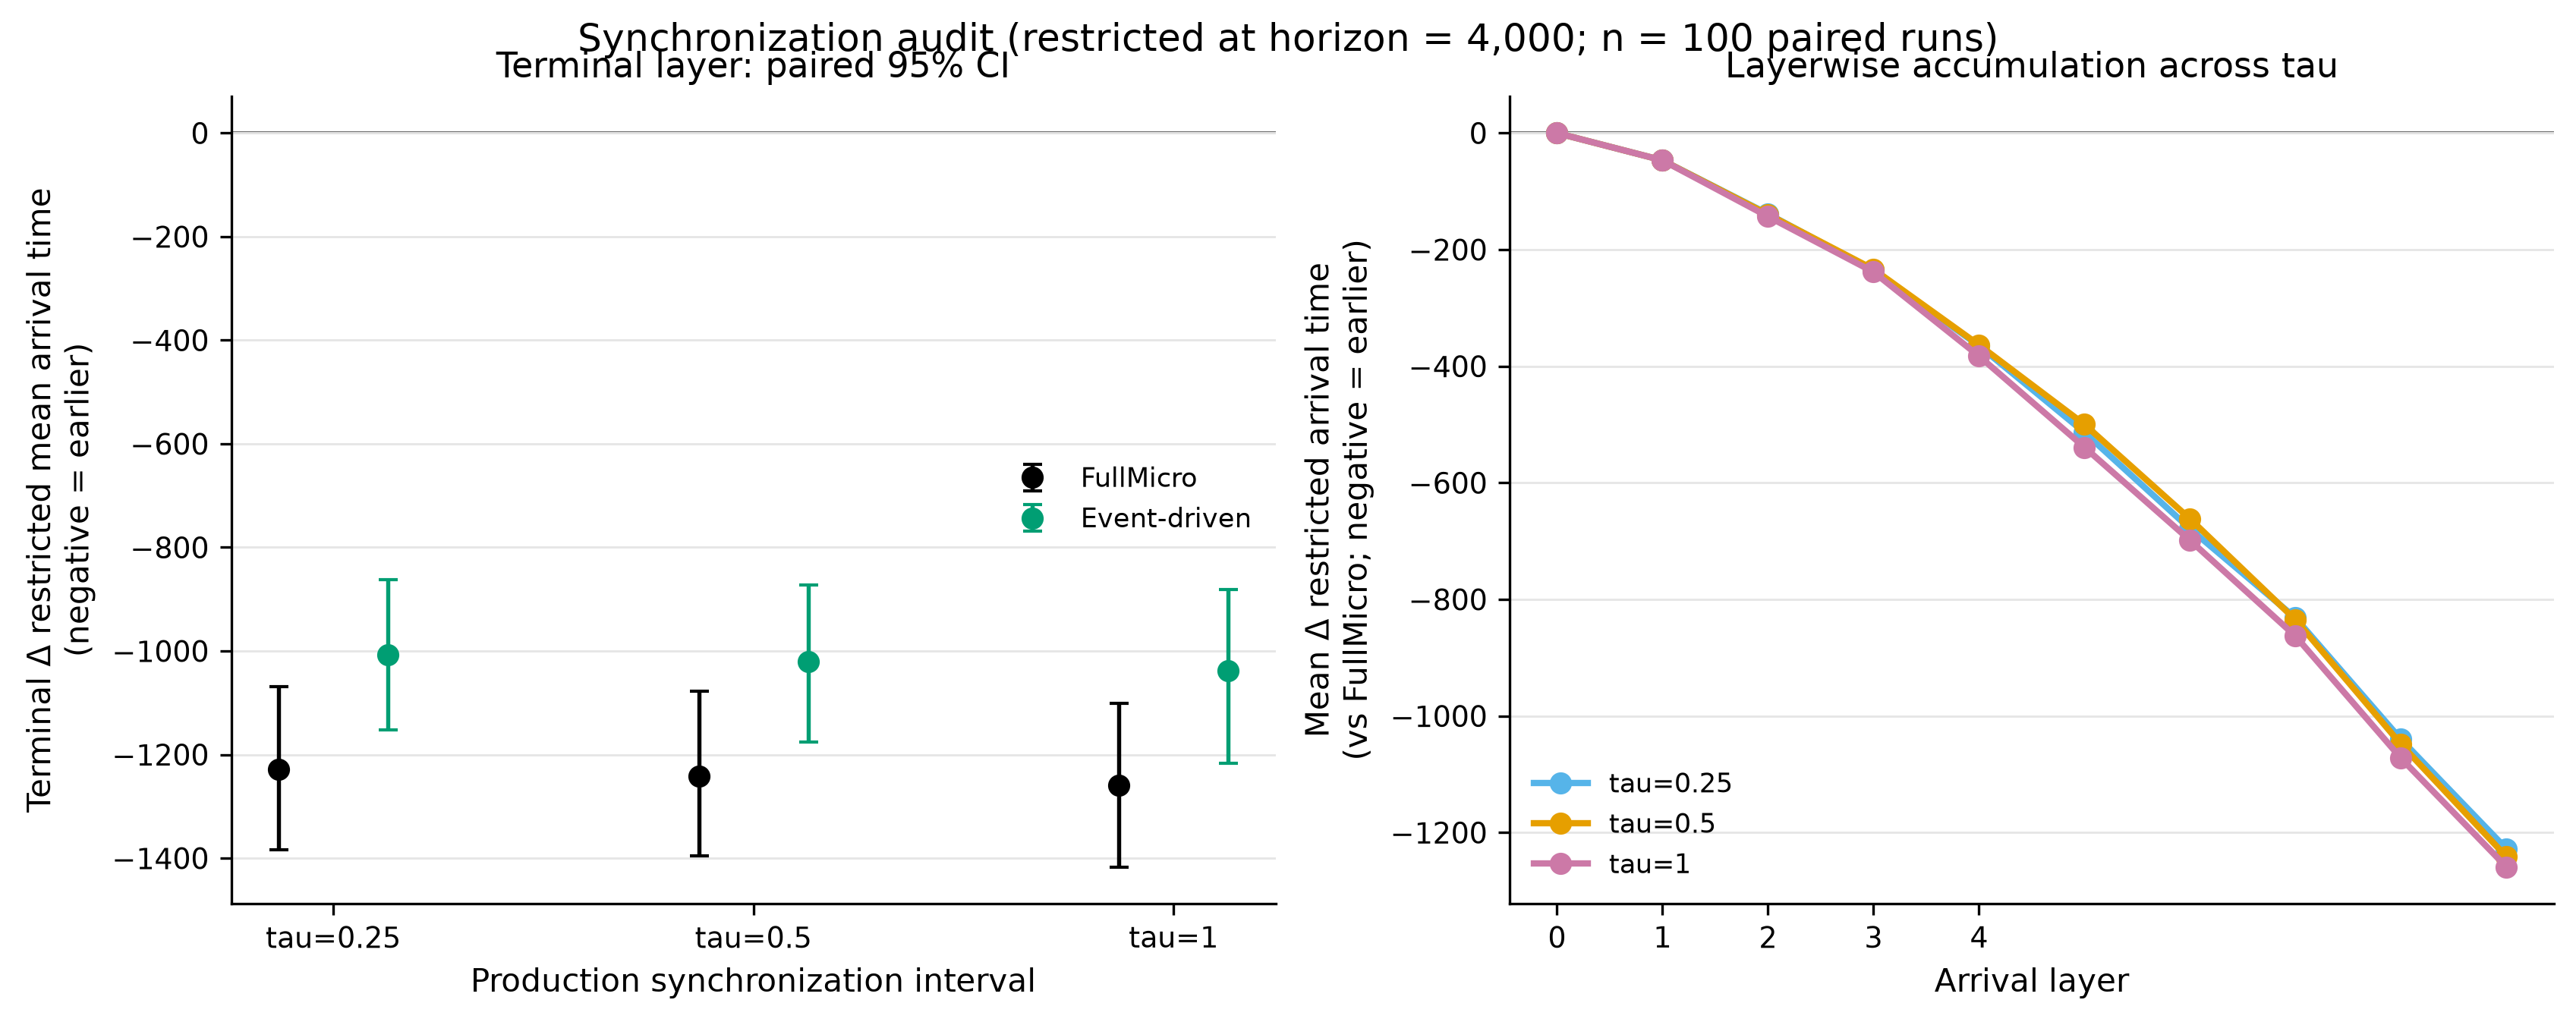
\includegraphics[width=0.94\linewidth]{figures/report_figure.png}
  \caption{Термінальна похибка та її накопичення за шарами для Full Micro,
  event-driven aggregate scheduler і production variants. Числові контрасти
  наведено в табл.~\ref{tab:full}--\ref{tab:layers}.}
  \label{fig:sync}
\end{figure}

\section{Аналіз та каузальна інтерпретація}\label{sec:interpretation}

Event-driven aggregate model уже має передчасне зміщення $-220.79$, сумісне
з rate/placement abstraction error. Production variants мають приблизно
$-1228$--$-1259$, тобто додають понад 1000 часових одиниць раннього зміщення
відносно event-driven reference. У цій конфігурації реалізаційна семантика є
великим окремим джерелом approximation error.

Зміна point estimate від $\tau=1$ до $0.25$ мала порівняно з відстанню всіх
production variants до event-driven path. Проте цей факт не є тестом
збіжності. Production і event-driven algorithms відрізняються семантикою
hazard accumulation, state updates та synchronization, тому аудит вимірює
їхню сукупну різницю, а не чисту quadrature error.

У шарі 1 зсув production і event-driven майже однаковий, але після кількох
меж production discrepancy накопичується (табл.~\ref{tab:layers} і
рис.~\ref{fig:sync}). Це узгоджується з повторним внесенням реалізаційної
різниці на кожному переході, але не визначає, яка саме внутрішня операція є
причиною.

\section{Значення для двошарової апроксимації та статті}\label{sec:paper}

\begin{itemize}
  \item Похибку production MicroMacro не можна приписувати лише aggregate
  hazard або placement.
  \item Механістичні ablation-висновки event-driven моделі не слід переносити
  на production implementation без перевірки семантики.
  \item У статті варто окремо показати model abstraction error (Full проти
  event-driven) та implementation discrepancy (production проти event-driven).
  \item Layerwise accumulation є необхідним діагностичним результатом:
  ранні шари приховують подальше розходження.
\end{itemize}

\section{Обмеження і твердження, яких слід уникати}\label{sec:limits}

\begin{enumerate}
  \item Перевірено лише $\tau=0.25$, $0.5$ і $1$; немає послідовності, що
  прямує до нуля. Не слід заявляти ані збіжність, ані незбіжність при
  $\tau\to0$.
  \item Прямих paired CI для $\tau=0.25$ проти $0.5$ або $1$ немає.
  Перекривання окремих CI не є тестом між-$\tau$ різниці.
  \item Це порівняння двох реалізаційних семантик, а не чистої quadrature rule
  за інших рівних умов.
  \item Одна SI-конфігурація й один горизонт не обґрунтовують універсального
  твердження про production MicroMacro.
  \item Completion 1 усуває цензурування лише в цьому наборі; за іншого
  горизонту RMST і completion слід аналізувати спільно.
  \item Аудит не оцінює runtime і не підтримує тверджень про прискорення.
\end{enumerate}

\section{Практичні рекомендації}\label{sec:recommendations}

\begin{enumerate}
  \item Узгодити semantics import scheduling, hazard accumulation і state
  synchronization з event-driven reference.
  \item Додати контрольовані unit/trajectory tests на одному
  міжспільнотному переході.
  \item Після семантичного узгодження провести окреме convergence study на
  ширшій логарифмічній сітці $\tau$ з прямими paired CI.
  \item У поточному рукописі називати production discrepancy похибкою
  реалізації, а не доказом неспроможності двошарової ідеї.
\end{enumerate}

\section{Відтворення}\label{sec:reproduction}

Runner: \path{extrascripts/run_synchronization_audit.py}. \\
Результати: \path{output/missing_experiments/synchronization_audit/full/summary.csv}
та \path{output/missing_experiments/synchronization_audit/full/arrivals.csv}. \\
Маніфест: \path{output/missing_experiments/synchronization_audit/full/manifest.json}. \\
Архівні референси: \path{output/ablation_hazard_placement/final_100/arrival_times.csv}
і \path{output/ablation_hazard_placement/final_100/runs.csv}.
Маніфест фіксує параметри, pairing, seed policy і SHA-256 runner/source.

\end{document}
